% Source: graduate-coursework/Research/Intro_to_Agents/handouts/Part2_Agent_Foundations.tex

\documentclass[border=4pt]{standalone}
\usepackage{amsmath}
\usepackage{amssymb}
\usepackage{tikz}
\usepackage{xcolor}
\usetikzlibrary{shapes.geometric, arrows.meta, positioning, fit, calc, backgrounds}

\definecolor{UofSCGarnet}{HTML}{73000a}
\definecolor{UofSCBlack}{HTML}{000000}
\definecolor{UofSCWhite}{HTML}{ffffff}
\definecolor{UofSCAtlantic}{HTML}{466A9F}
\definecolor{UofSCCongaree}{HTML}{1F414D}
\definecolor{UofSCRose}{HTML}{CC2E40}
\definecolor{UofSCHorseshoe}{HTML}{65780B}
\definecolor{UofSCGrass}{HTML}{CED318}
\definecolor{UofSCHoneycomb}{HTML}{A49137}
\definecolor{UofSCDarkGarnet}{HTML}{570008}
\definecolor{UofSCAzalea}{HTML}{844247}
\definecolor{UofSC90Black}{HTML}{363636}
\definecolor{UofSC70Black}{HTML}{5C5C5C}
\definecolor{UofSC50Black}{HTML}{A2A2A2}
\definecolor{UofSCWarmGrey}{HTML}{676156}
\definecolor{UofSCSandstorm}{HTML}{FFF2E3}

\tikzset{
    % Box styles with sharp corners
    component/.style={
        rectangle,
        draw=UofSCBlack,
        fill=UofSCWhite,
        thick,
        minimum width=3cm,
        minimum height=1cm,
        align=center,
        font=\small
    },
    component garnet/.style={
        component,
        fill=UofSCGarnet!10,
        draw=UofSCGarnet,
        thick
    },
    component atlantic/.style={
        component,
        fill=UofSCAtlantic!10,
        draw=UofSCAtlantic,
        thick
    },
    component congaree/.style={
        component,
        fill=UofSCCongaree!10,
        draw=UofSCCongaree,
        thick
    },
    loop node/.style={
        rectangle,
        draw=UofSCGarnet,
        fill=UofSCGarnet!15,
        thick,
        minimum width=2.5cm,
        minimum height=1.2cm,
        align=center,
        font=\footnotesize\bfseries
    },
    decision/.style={
        diamond,
        draw=UofSCBlack,
        fill=UofSCHoneycomb!20,
        thick,
        minimum width=2cm,
        minimum height=1.5cm,
        align=center,
        font=\footnotesize,
        aspect=2
    },
    arrow style/.style={
        ->,
        >=Stealth,
        thick,
        UofSCBlack
    },
    biarrow style/.style={
        <->,
        >=Stealth,
        thick,
        UofSCBlack
    }
}

\begin{document}
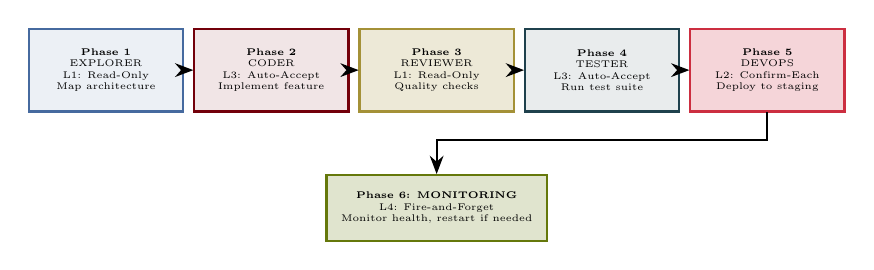
\begin{tikzpicture}[scale=0.7, transform shape]
        % Phases as a pipeline
        \node[component atlantic, minimum width=2.8cm, minimum height=1.5cm, font=\tiny, align=center] (p1) at (-6, 0) {
            \textbf{Phase 1}\\
            EXPLORER\\
            L1: Read-Only\\
            Map architecture
        };

        \node[component garnet, minimum width=2.8cm, minimum height=1.5cm, font=\tiny, align=center] (p2) at (-3, 0) {
            \textbf{Phase 2}\\
            CODER\\
            L3: Auto-Accept\\
            Implement feature
        };

        \node[component, fill=UofSCHoneycomb!20, draw=UofSCHoneycomb, minimum width=2.8cm, minimum height=1.5cm, font=\tiny, align=center] (p3) at (0, 0) {
            \textbf{Phase 3}\\
            REVIEWER\\
            L1: Read-Only\\
            Quality checks
        };

        \node[component congaree, minimum width=2.8cm, minimum height=1.5cm, font=\tiny, align=center] (p4) at (3, 0) {
            \textbf{Phase 4}\\
            TESTER\\
            L3: Auto-Accept\\
            Run test suite
        };

        \node[component, fill=UofSCRose!20, draw=UofSCRose, minimum width=2.8cm, minimum height=1.5cm, font=\tiny, align=center] (p5) at (6, 0) {
            \textbf{Phase 5}\\
            DEVOPS\\
            L2: Confirm-Each\\
            Deploy to staging
        };

        % Arrows
        \draw[arrow style] (p1) -- (p2);
        \draw[arrow style] (p2) -- (p3);
        \draw[arrow style] (p3) -- (p4);
        \draw[arrow style] (p4) -- (p5);

        % Monitoring below
        \node[component, fill=UofSCHorseshoe!20, draw=UofSCHorseshoe, minimum width=4cm, minimum height=1.2cm, font=\tiny, align=center] (p6) at (0, -2.5) {
            \textbf{Phase 6: MONITORING}\\
            L4: Fire-and-Forget\\
            Monitor health, restart if needed
        };

        \draw[arrow style] (p5.south) -- ++(0,-0.5) -| (p6.north);
    \end{tikzpicture}
\end{document}
